\documentclass[a4paper]{article}
\usepackage{amssymb, amsmath}
\usepackage{graphicx}
\begin{document}
\section{Linear Regression}
\subsection{Linear Regression Basic}
\noindent{\bf a. Assumption}\\
1)	Weak exogeneity. \\
the predictor variables x can be treated as fixed values, rather than random variables.\\
2)	Linearity. \\
The mean of the response variable is a linear combination of the parameters (regression coefficients) and the predictor variables. \\
3)	Constant variance (a.k.a. homoscedasticity). \\
Different values of the response variable have the same variance in their errors, regardless of the values of the predictor variables. \\
4)	Independence of errors. \\
This assumes that the errors of the response variables are uncorrelated with each other.\\
5)	Lack of perfect multicollinearity in the predictors. \\
For standard least squares estimation methods, the design matrix X must have full column rank p; otherwise, we have a condition known as perfect multicollinearity in the predictor variables\\

\noindent{\bf b. Matrix representation}\\
$Y = Hw + \epsilon$\\
where Y is $N \times 1$, H is $N \times D$, w is $D \times 1$, $\epsilon$ is $N \times 1$.\\

\noindent{\bf c. Cost Function}\\
\begin{align}
L({\bf w}) = \sum_{i=1}^N ({\bf y} - {\bf \hat y})^2
     = \sum_{i=1}^N ({\bf y} - {\bf Hw})^2	
\end{align}

\noindent{\bf d. Analytical Solution}\\
\begin{align}
	grad L({\bf w}) = -2 {\bf X}^T({\bf y}-{\bf Hw}) =0 \\
	{\bf w} = ({\bf H}^{T} {\bf H})^{-1} {\bf H}^{T} {\bf y} \\
\end{align}

\noindent{\bf e. Analysis of Analytical Solution}\\
1) To have $(H^{T} H)^{-1}$ invertible, the number of observations > the number of features.\\
2) Requires matrix inverse which is $O(n^3)$, too computationally intensive.\\
3) That��s why we need to seek for numerical solution, like gradient descent.\\

\noindent{\bf f. Gradient descent algorithm}\\
Init $w^{1} = 0$\\
while $||\frac{\partial L(\hat w)}{\partial \hat w}||_2 > \epsilon$\\
For i= 1 to D(loop of features)\\
\indent $\,   \frac{\partial L(w_j)}{\partial w_j} = -2 \sum_i^{N} H_{ij}(y_i - \hat y_i (w^{t}))$\\
\indent $\,    w^{j+1}_j = w^{j+1}_j - \eta * \frac{\partial L(w_j)}{\partial w_j};$\\
t= t+1;\\
In order to write the gradient in matrix notation, note\\
\begin{align*}
	\frac{\partial L(w_j)}{\partial w_j} 
	 = & -2 \sum_i^{N} H_{ij}(y_i - \hat y_i (w^{t}))$\\
	 = & -2 \left( \begin{array}{ccccc} H_{1j} & H_{2j} & H_{3j} &. . . &H_{Nj} \end{array} \right)
										 \left( \begin{array}{c}
											y_1 - \hat y_1 (w^{t}) \\
										  	y_2 - \hat y_2 (w^{t}) \\
										   	y_3 - \hat y_3 (w^{t}) \\
										    ... \\
										    y_N - \hat y_N (w^{t}) \\
										\end{array} \right)
\end{align*}


	\left( \begin{array}{c} \frac{\partial L(w_1)}{\partial w_1} \\
	\frac{\partial L(w_2)}{\partial w_2} \\
	\frac{\partial L(w_3)}{\partial w_3} \\
	...\\
	\frac{\partial L(w_5)}{\partial w_5} \\
	\end{array} \right)
		 = -2 \left( \begin{array}{ccccc}
		 H_{11} & H_{21} & H_{31} &. . . &H_{N1}\\
		 H_{22} & H_{22} & H_{32} &. . . &H_{N2}\\		 									
		 H_{13} & H_{23} & H_{33} &. . . &H_{N3}\\
		 ...\\
		 H_{1D} & H_{2D} & H_{3D} &. . . &H_{ND}\\

		\end{array} \right)
										 \left( \begin{array}{c}
											y_1 - \hat y_1 (w^{t}) \\
										  	y_2 - \hat y_2 (w^{t}) \\
										   	y_3 - \hat y_3 (w^{t}) \\
										    ... \\
										    y_N - \hat y_N (w^{t}) \\
										\end{array}
										 \right)

\begin{align*}
	 \frac{\partial L( {\bf w})}{\partial {\bf w}} = -2 H^T ({\bf y} - \hat {\bf y}({\bf w}^{t})  )\\
\end{align*}


\subsection{Performance Assessment/Model Selection}
\noindent{\bf a. Training/validation/testing data split} \\
1)	Fit the model parameters using the training data \\
2)	Select the model that minimize the error function on the validation data set \\
3)	Use the error on the test set as a generalization assessment of the model \\

\noindent{\bf b. K fold Cross Validation}\\
K fold cross validation applies in the situation where there is not so much data available so we use different portion of the data as validation set and we evaluate the model multiples times. The method has the following setups:\\
1)	Shuffle the data \\
2)	Divide the data into k set, called data[1] data[2]��..data[k] \\
3)	For(int i =0; i $\leq$k; i++) \\
\{\\  
\indent use data[i] as validation set,\\
\indent The rest data as training set, \\
\indent Fit the model, get $RSS_i$. \\
\}\\
For example, we partition the data into 10 sets, called $P_1$ to $P_{10}$. First we use $P_1$ as validation, the rest as training. Second we use $P_2$ as validation, the rest as training. Third we use $P_3$ as validation, the rest as training. \\
4)	Average RSS_{Aver}($\lambda$), \\
5)	Repeat the same procedure 1-4 for models. \\
6)	Pick the model that gives the least average $RSS_{Aver}$. \\
7)	Use this model to train the entire data set.\\


\noindent {\bf c. Understanding Bias and Variance Tradeoff}\\
Define $f_{\hat w}(x)$ as the fitted value average over all possible values of w, then\\
The mean square error\\
\begin{align*}
	&MSE(f_{\hat w(train)} (x))\\
&= E_{training}((f_{w(true)}(x) - f_{\hat w}(x))^2)\\
&= E_{training}(   (    (f_{w(true)}(x) - f_{\bar w}(x)) +
 (f_{\bar w}(x) - f_{\hat w}(x)   )^2)\\
&= E((f - \bar f)^2) +2E((f - \bar f)(\bar f - \hat f))
     + E(\bar f - \hat f)^2\\
&E((f -\bar f)^2) = bias^2(f)\\
&E(\bar f - \hat f)^2 = var(\hat f)\\
&2E((f-\bar f)(\bar f- \hat f)) = 0\\
&MSE(f_{\hat w(train)} (x)) = bias^2 f + var(\hat f)\\
\end{align*}

\noindent 1) Conclusion\\
High bias leads to under fitting\\
High variance leads to over fitting\\

\noindent 2) A plot which shows how training error and validation error changes as the model goes more complex\\
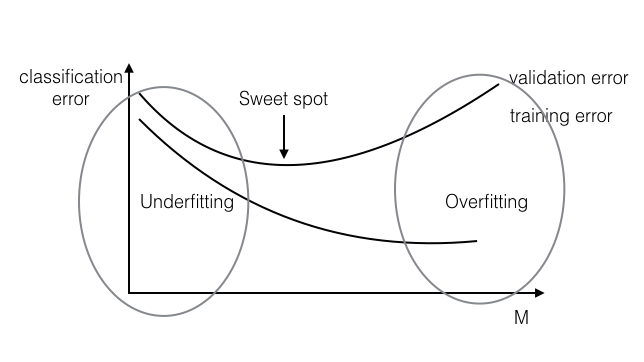
\includegraphics[scale =0.4]{1.png}\\
{\tiny http://www.cs.cornell.edu/courses/cs4780/2015fa/web/lecturenotes/lecturenote13.html}


\noindent{\bf d. Debugging Learining Algorithm Tricks}\\
1) Getting more training examples would be likely to fix high variance\\
2) Smaller sets of features would be likely to fix high variance\\
3) Getting additional feature would be likely to fix high bias\\
4) Decrease penalty parameter would be likely to fix high bias\\
5) Increase penalty parameter would be likely to fix high variance\\

\subsection{Ridge and Lasso Regression}
{\bf a. Definition}\\
Ridge uses two norm as penalty and add it into the cost function, $\lambda \sum w_i^2$\\
Lasso uses one norm as penalty and add it into the cost function, $\lambda \sum \abs(w_i)$\\
{\bf b. Method}\\  
1) Ridge regression: Gradient descent\\
\begin{align*}
	{\bf Y} = {\bf Hw} + {\bf \epsilon} \\
	L({\bf w})= \sum_{i=1}^N ({\bf y} - {\bf Hw})^2 +  \lambda \sum w_i^2 \\
	\grad Loss = -2 {\bf H}^T({\bf y}-{\bf Hw})+ 2 \lambda w \\
\end{align*}
Step update:  
for $j\neq 0$:\\
\begin{align*}
{\bf w}^{(t+1)} = {\bf w}^{(t)} - \eta (-2 {\bf H}^T({\bf y}-{\bf H*w}) - 2 \lambda {\bf w})\\
\end{align*}
if j =0, as we do not need to add penalty to the constant term:
\begin{align*}
{\bf w}^{(t+1)} = {\bf w}^{(t)} - \eta (-2 {\bf H}^T({\bf y}-{\bf H*w}) )
\end{align*}
2) Ridge regression: Analytical\\
\begin{align*}
	w = (H^T H + \lambda \left( \begin{array}{ccccc}
		0 & 0 & 0 & 0 & 0 \\
		0 & 1 & 0 & 0 & 0 \\
		0 & 0 & 1 & 0 & 0 \\
		0 & 0 & 0 & 1 & 0 \\
		0 & 0 & 0 & 0 & 1 \\
	\end{array} \right)  )^{-1} X^TY
\end{align*}
3) Lasso regression: Coordinate descent\\
\begin{align*}
	L({\bf w}) = \sum_{i=1}^N ({\bf y} - {\bf Hw})^2 \\
	L^{'}({\bf w}) = \sum_{i=1}^N ({\bf y} - {\bf Hw})^2 +  \lambda \sum \abs{w_i} \\
\end{align*}
\begin{align*}
	&\frac{\partial L(\bf w)}{\partial w_j}\\
=  & -2 \sum_{i=1} ^{N} h_{ij}(y_i - \sum_{j=1}^D w_j H_{ji})\\
=  & -2 \sum_{i=1} ^{N} h_{ij}(y_i - \sum_{k \neq j} w_k H_{ki}) \\
+ 2 w_j \sum_{i=1}^{N} h_{ij} ^2 \\
\end{align*}
We let this equal to 
\begin{align*}
-2 \rho_j + 2 w_j z_j	
\end{align*}
The gradient of the penalty term\\
\begin{align*}
 &	\lambda \frac{\partial |w_j|}{\partial w_j} \\
=& -\lambda  \text{ when } w_j <  0 \\
 & [-\lambda, \lambda] \text{ when }w_j =  0 \\
 & \lambda \text{ when } w_j >  0 \\
\end{align*}

\begin{align*}
	&\frac{\partial L^{'}(\bf w)}{\partial w_j}\\
= & -2 \rho_j + 2 w_j z_j -\lambda \text{ when } w_j <  0 \\
  & [-2 \rho_j -\lambda, -2 \rho_j + \lambda] \text{ when } w_j =  0 \\
  &   -2 \rho_j + 2 w_j z_j + \lambda \text{ when } w_j >  0 \\
\end{align*}
So
\begin{align*}
w_j & = \frac{\rho_j + \lambda/2}{z_j}  \text{ if } \rho_j < - \lambda/2\\
w_j & = 0  \text{ if }  - \lambda/2 < \rho_j <  \lambda/2 \\
w_j & = \frac{\rho_j - \lambda/2}{z_j}  if \rho_j >  \lambda/2 \\
\end{align*}
3) Comparison\\
\begin{tabular}{ l | l | l | l }
				  &  Ridge & Lasso & Comment \\
				  \hline
  Model selection &   No & Yes & By drawing the contour\\ 
  					& & &parameter in lasso shrinks to zero \\
  					\hline
  Has analytical, and unique solution & Yes & No & Derivative is not continuous in Lasso\\
  \hline
  Stable  & Yes & No &  Ridge can deal better in colinearity \\
\end{tabular}
\\
\\
\noindent Plot of the contours of the original cost function(purple) and penalty term(blue) for both ridge and lasso regression. The tangent point between purple and blue curve is the solution.\\
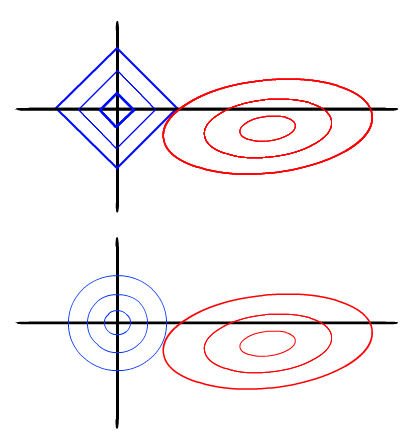
\includegraphics[scale =0.4]{2.png}\\
{\tiny https://stats.stackexchange.com/questions/30456/geometric-interpretation-of-penalized-linear-regression}\\
\\
\noindent 4) Usage
We usually use Lasso to select parameters, then use ridge to find the optimal solution.\\
\end{document}